\begin{tikzpicture}
\begin{scope}
% ratio removal
\clip (0,2.95) rectangle (8,9.8);
\node[anchor=south west,inner sep=0] at (0,0) {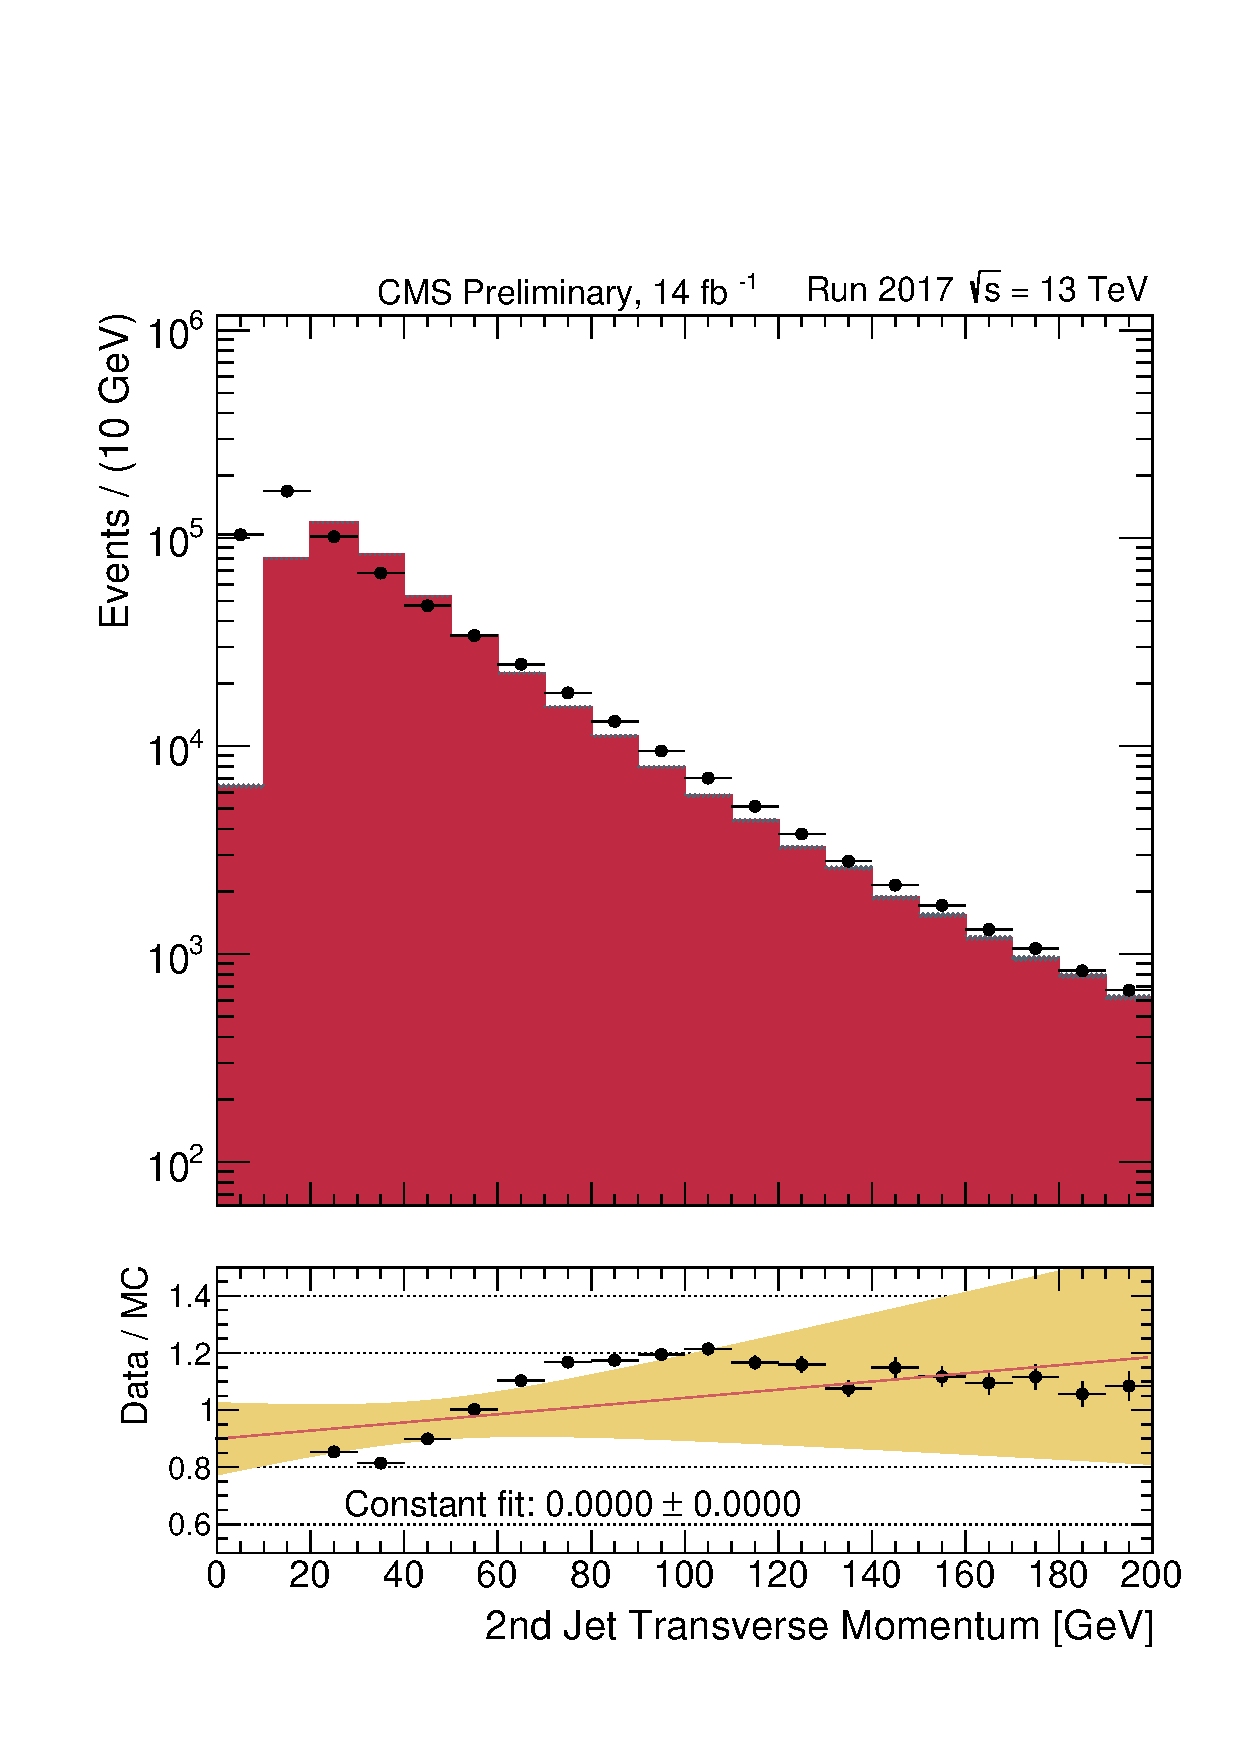
\includegraphics[width=8cm]{\PhDthesisdir/plots_and_images/my_plots/JERC/distributions/2018/source/ptSecondJet_log.pdf}};

% above txt
\fill [white] (0, 9.37) rectangle (8,9.7);
\draw (7.65, 9.6) node [left] {\footnotesize Run 2018 ABCD, \SI{59}{\femto\barn^{-1}} (\SI{13}{\TeV})};

% masks
\fill [white] (1, 0) rectangle (8,.95);
\fill [white] (0, 1) rectangle (1.15,9.4);

% X axis
\foreach \val in {0, 20, ..., 200}{
\draw ({1.2+(7.53-1.2)*(\val)/(200)}, .85) node {\small \val};
}
\draw (7.5, .45) node [left] {\normalsize $\pT^\text{jet 2}$ (\SI{}{\GeV})};

% Y axis
\foreach \pos/\val in {3/10^3, 4/10^4, 5/10^5, 6/10^6}{
\draw (1.3, {4.6+(\pos-3)/(6-3)*(8.6-4.6)}) node [left] {\small $\val$};
}
\draw (.25, 9.55) node [left, rotate=90] {\normalsize Nombre d'événements / \SI{10}{\GeV}};

\end{scope}
% new X axis
\foreach \val in {0, 20, ..., 200}{
\draw ({1.2+(7.53-1.2)*(\val)/(200)}, .85+2.3) node {\small \val};
}
\draw (7.5, .45+2.3) node [left] {\normalsize $\pT^\text{jet 2}$ (\SI{}{\GeV})};

% CMS disclaimer
\draw (1.05, 9.6) node [right] {\footnotesize CMS Data};
\draw (7, 8.9) node [left] {\emph{Own work}};
\end{tikzpicture}
